\documentclass[a4paper,12pt]{article}

\title{Chapter 4. Interacting Fields and Feynman Diagrams\\
4-4. Feynman Diagrams}
\date{各種SNS\\
    X (旧 Twitter): \href{https://x.com/miya_max_study}{@miya\_max\_study}\\
    Instagram : \href{https://www.instagram.com/daily_life_of_miya/}{@daily\_life\_of\_miya}\\
    YouTube : \href{https://www.youtube.com/@miya-max-active}{@miya-max-active}
    }
\author{Max Miyazaki}

\usepackage{amsmath}
\usepackage{amssymb}
\usepackage{ascmac}
\usepackage{amsthm}
\usepackage{amsfonts}
\usepackage{enumitem}
\usepackage{color}
\usepackage[dvipdfmx]{graphicx}
\usepackage{float}
\usepackage{bm}
\usepackage{here}
\usepackage{simpler-wick}
\usepackage{abstract}
\usepackage{tikz}
\usetikzlibrary{shapes.geometric, arrows.meta, positioning}
\usepackage{indentfirst}
\usepackage[utf8]{inputenc}
\usepackage{fix-cm}
\usepackage{wrapfig}
\pagenumbering{arabic}
\usepackage{url}
\usepackage{xcolor}
\usepackage[most]{tcolorbox}
\usepackage{framed}
\usepackage[dvipdfmx]{hyperref}
\hypersetup{
 setpagesize=false,
 bookmarksnumbered=true,
 colorlinks=true,
 linkcolor=blue
}

% Define braket-like commands
\newcommand{\bra}[1]{\left\langle #1\right|}
\newcommand{\ket}[1]{\left|#1\right\rangle}
\newcommand{\braket}[2]{\left\langle #1\middle|#2\right\rangle}
\newcommand{\brakets}[3]{\left\langle #1\middle| #2 \middle|#3 \right\rangle}

\renewcommand{\arraystretch}{2.1}


\setlength{\textwidth}{16cm}
\setlength{\textheight}{25cm}
\setlength{\oddsidemargin}{0cm}
\setlength{\evensidemargin}{0cm}
\setlength{\topmargin}{-2cm}

\begin{document}
\maketitle

\vspace{1cm}
\begin{abstract}
    このノートはPeskin\&Schroederの``An Introduction to Quantum Field Theory''の第4章の4節をまとめたものである. 要点や個人的な追記, 計算ノート的なまとめを行っているが, それらはすべて原書の内容を出発点としている. 参考程度に使っていただきたいが, このノートは私の勉強ノートであり, そのままの内容をそのまま鵜呑みにすると間違った理解を招く可能性があることをご了承ください. ぜひ原著を手に取り, その内容をご自身で確認していただくことを推奨します. てへぺろ v$({\hat{\cdot}_\partial \hat{\cdot}})$v
\end{abstract}
    
    

\newpage
\color{blue}
\section*{概要}
\begin{itemize}
  \item \textbf{出発点}
  \begin{itemize}
    \item 相関関数の摂動展開では、自由場の時間順序積の真空期待値を計算する必要がある.
    \item 例: $\langle 0| T\{\phi(x_1)\phi(x_2)\cdots \phi(x_n)\}|0\rangle$.
  \end{itemize}

  \item \textbf{場の分解}
  \begin{itemize}
    \item 自由場を正の周波数部分と負の周波数部分に分ける:
    \[
      \phi_I(x) = \phi_I^+(x) + \phi_I^-(x),
    \]
    \item 性質: $\phi_I^+(x)|0\rangle=0$, $\langle 0|\phi_I^-(x)=0$.
  \end{itemize}

  \item \textbf{縮約の定義}
  \begin{itemize}
    \item 二つの場 $\phi(x), \phi(y)$ の縮約を
    \[
      \wick{\c1 \phi(x)\, \c1 \phi(y)}
      \equiv [\phi^+(x), \phi^-(y)]
    \]
    と定義する.
    \item これはファインマン伝播子 $D_F(x-y)$ に等しい.
  \end{itemize}

  \item \textbf{時間順序と正規順序の関係}
  \begin{itemize}
    \item 二点の場合:
    \[
      T\{\phi(x)\phi(y)\} = N\{\phi(x)\phi(y)\} 
      + \wick{\c1 \phi(x)\, \c1 \phi(y)}.
    \]
    \item 時間順序積 = 正規順序積 + 縮約.
  \end{itemize}

  \item \textbf{ウィックの定理(一般化)}
  \begin{itemize}
    \item 任意個の場に対して:
    \[
      T\{\phi(x_1)\phi(x_2)\cdots\phi(x_m)\}
      = N\{\phi(x_1)\phi(x_2)\cdots\phi(x_m)\} 
      + \text{すべての可能な縮約}.
    \]
    \item 「すべての可能な縮約」とは、場をペアに縮約するあらゆる組み合わせを含む.
  \end{itemize}

  \item \textbf{具体例 ($m=4$ の場合)}
  \begin{itemize}
    \item $T\{\phi_1\phi_2\phi_3\phi_4\}$ は正規順序項に加えて6通りの縮約を持つ.
    \item 例:
    \[
      \wick{\c1 \phi_1 \c1 \phi_2}\phi_3\phi_4,\quad
      \wick{\c1 \phi_1 \c1 \phi_3}\phi_2\phi_4,\quad
      \wick{\c1 \phi_1 \c1 \phi_4}\phi_2\phi_3,\quad \dots
    \]
    \item 真空期待値をとると、縮約が残らない項は消え、完全に縮約された3通りの項だけが残る.
  \end{itemize}

  \item \textbf{結果(4点関数の真空期待値)}
  \[
    \langle 0|T\{\phi_1\phi_2\phi_3\phi_4\}|0\rangle
    = D_F(x_1-x_2)D_F(x_3-x_4)
    + D_F(x_1-x_3)D_F(x_2-x_4)
    + D_F(x_1-x_4)D_F(x_2-x_3).
  \]

  \item \textbf{意義}
  \begin{itemize}
    \item 複雑な相関関数を、伝播子(ファインマン伝播子)の積の和として計算可能にする.
    \item 後のファインマン図の構築の基礎となる.
  \end{itemize}
\end{itemize}


\newpage
\color{black}
\section*{4.4 Feynman Diagrams}

ウィックの定理を使えば、次のような式

\[
\langle 0| T\{\phi_I(x_1)\phi_I(x_2)\cdots \phi_I(x_n)\} |0 \rangle
\]

を、ファインマン伝播子の積の和に変形できる。  
ここで我々は、このような式の図式的解釈を発展させる準備が整った。  
まず、4つの場がすべて異なる時空点にある場合を考えよう。これは式 (4.40) で既に計算した。  
各点 $x_1$ から $x_4$ を点で表し、各因子 $D_F(x-y)$ を $x$ と $y$ を結ぶ線で表すことにする。  

すると、式 (4.40) は3つの図(\textbf{ファインマン図} と呼ばれる)の和として表せる:
\begin{align*}
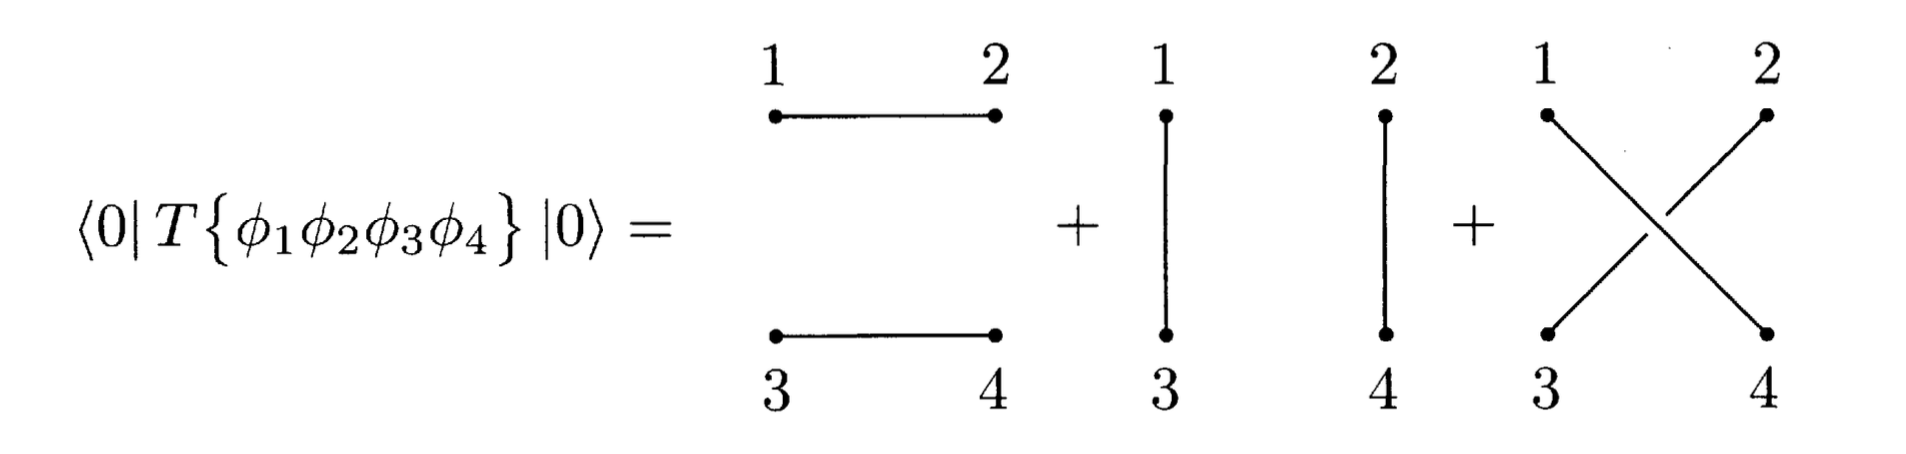
\includegraphics[width=0.9\textwidth]{figures/4.42.png}\tag{4.42} \label{4.42}
\end{align*}
これは直接的に測定できる量ではないが、図は重要な解釈を与えている。  
すなわち、粒子が2つの時空点で生成され、それぞれ他の点へ伝播し、そこで消滅する、という描像である。  
この過程は3通りあり、点をペアに接続する3つの異なる方法に対応する。  
全過程の振幅は3つの図の和である。  

---

さらに興味深いのは、同じ時空点に複数の場が現れる場合である。  
二点関数 $\langle \Omega|T\{\phi(x)\phi(y)\}|\Omega\rangle$ に戻り、式 (4.31) を使おう。  
分母は最後まで無視し、分子を級数展開すると次を得る:

\[
\langle 0|T\{\phi(x)\phi(y) + \phi(x)\phi(y)(-i)\int dt\, H_I(t) + \cdots \}|0\rangle .
\tag{4.43}
\]

最初の項は自由場の結果であり、

\[
\langle 0|T\{\phi(x)\phi(y)\}|0\rangle = D_F(x-y).
\]

二番目の項は $\phi^4$ 理論において次のようになる:

\[
\langle 0|T\{\phi(x)\phi(y)(-i)\int dt \int d^3z \frac{\lambda}{4!}\phi^4(z)\}|0\rangle .
\]

これは

\[
= \langle 0|T\{\phi(x)\phi(y)\}\left(\frac{-i\lambda}{4!}\right)\int d^4z\, \phi(z)\phi(z)\phi(z)\phi(z)|0\rangle
\]

と書き直せる。  

ここでウィックの定理を適用する。$\phi$ の6つの演算子をペアに縮約するあらゆる方法に対して項が得られる。  
縮約の仕方は15通りあるが、実際には2種類だけが異なる。  
$\phi(x)$ を $\phi(y)$ と縮約すれば、残りの4つの $\phi(z)$ を互いに縮約する3通りの方法があり、それらはすべて同一の寄与を与える。  
別の可能性は、$\phi(x)$ を $\phi(z)$ の1つと縮約する(4通り)、同様に $\phi(y)$ を $\phi(z)$ と縮約する(3通り)、さらに残りの2つの $\phi(z)$ 同士を縮約する(1通り)。  
これらは12通りであり、すべて同一の寄与を与える。  

したがって次を得る:

\[
\begin{aligned}
\langle 0|T\{\phi(x)\phi(y)(-i)\int dt \int d^3z \tfrac{\lambda}{4!}\phi^4(z)\}|0\rangle
&= 3\cdot \left(\tfrac{-i\lambda}{4!}\right) D_F(x-y)\int d^4z\, D_F(z-z)D_F(z-z) \\
&\quad + 12\cdot \left(\tfrac{-i\lambda}{4!}\right)\int d^4z\, D_F(x-z)D_F(y-z)D_F(z-z).
\end{aligned}
\tag{4.44}
\]

この表現を、各項をファインマン図として理解するとさらに分かりやすい。再び各収縮項 $D_F$ を線として描き、各点をドットとして表す。だが今回は「外部点」$x, y$ と「内部点」$z$ を区別しなければならない。各内部点は因子 $\left(-i\lambda\right)\int d^4z$ と対応している。定数因子は今は気にしない。これらのルールを用いると、式 (4.44) は次の二つの図の和として表される:

\begin{equation*}
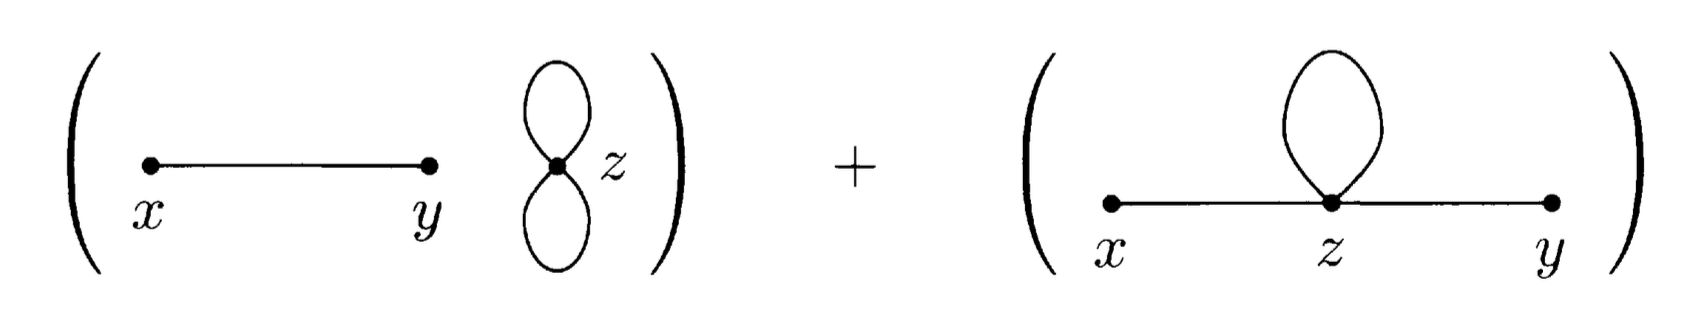
\includegraphics[width=0.9\textwidth]{figures/4.44.png}\tag{4.44} \label{4.44}
\end{equation*}


これらの図における線を \textbf{伝播子 (propagator)} と呼ぶ。なぜならそれらが伝播振幅 $D_F$ を表しているからである。内部点、すなわち4本の線が交わる点を \textbf{頂点 (vertex)} と呼ぶ。$D_F(x-y)$ が $x$ と $y$ の間で自由クライン・ゴルドン粒子が伝播する振幅であるように、これらの図は解析式を「粒子が生成され、伝播し、消滅する過程」として解釈するものであり、時空での物理過程を視覚的に示す。

次に、より複雑な収縮を考えてみよう。これは相関関数展開における $\lambda^3$ の項に由来する:

\[
\begin{aligned}
\langle 0| T\{\phi(x)\phi(y)\} 
\frac{1}{3!}\left(-i\frac{\lambda}{4!}\right)^3 
\int d^4z\, d^4w\, d^4u \;
\phi(z)^4 \phi(w)^4 \phi(u)^4
|0 \rangle .
\end{aligned}
\]
\textcolor{red}{ここの数式修正}
\[
= \frac{1}{3!}\left(-i\frac{\lambda}{4!}\right)^3
\int d^4z\, d^4w\, d^4u \;
D_F(x-z)D_F(z-z)D_F(z-w)
D_F(w-y)D_F(z-u)D_F(u-y).
\tag{4.45}
\]

この表現を与える「異なる」収縮の数は非常に大きい:

\[
3! \times \frac{4\cdot 3}{2} \times 4\cdot 3\cdot 2 \times 4\cdot 3 \times \frac{1}{2}
= 10{,}368 .
\]

これは14個の演算子に対する完全な収縮 135,135 通りのうちおよそ $1/13$ に相当する。  
この特定の収縮の構造は、次の \textbf{「サボテン (cactus) 図」} として表現できる:

\begin{equation*}
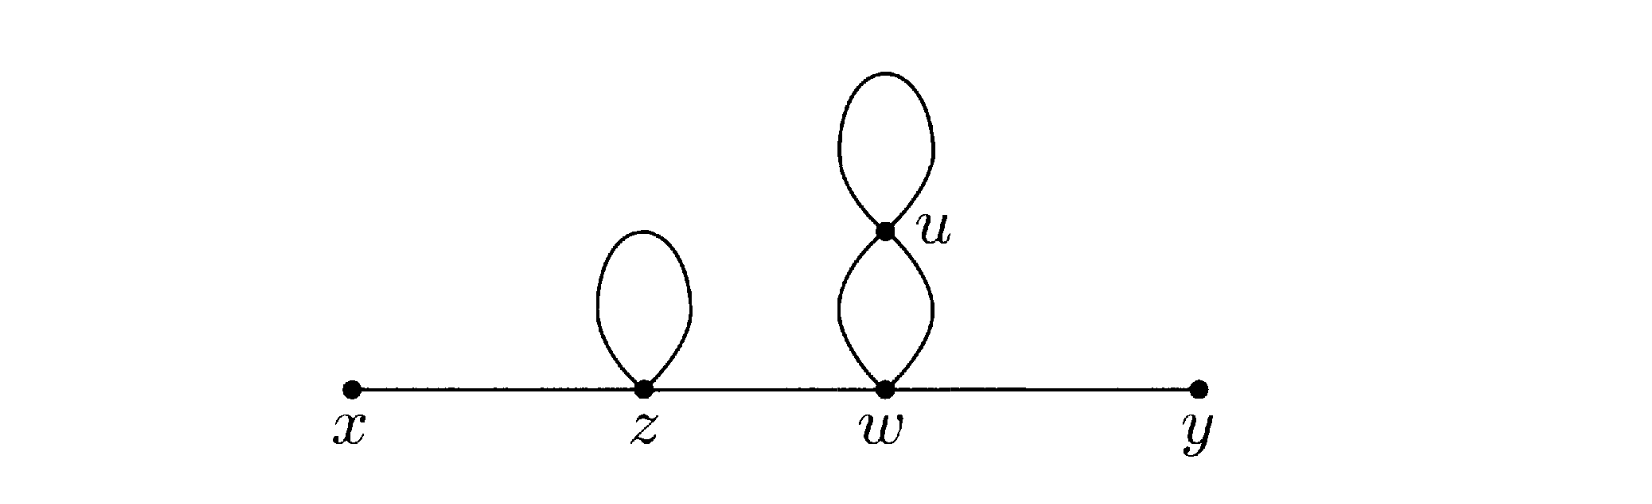
\includegraphics[width=0.9\textwidth]{figures/4.45.png}\tag{4.45} \label{4.45}
\end{equation*}

自明な理由により、この1枚の図が 10,368 個の全く同一の寄与の総和を表すものとするのが慣例である。

実際には、まず図を描き、その図を助けに解析的な式を書き下すのが常である。  
しかしここで問題が生じる:全体の定数因子は何か?  
もちろん、先ほどと同じように計算してもよい。すなわち、各頂点に対して因子 $\int d^4z (-i\lambda)$ を対応させ、テイラー展開からの $1/n!$ を入れる。  
そして積の展開で組合せ係数を数える。だがテイラー級数からの $1/n!$ は常にキャンセルされるため、これを無視できる。  
さらに、典型的な頂点は4本の線が入るが、この $4!$ は収縮の置換から出てくる。したがって頂点ごとに $4!$ を含める必要はなく、  
結局、各頂点に $(-i\lambda)\int d^4z$ を対応させるのが慣習である。これが $\phi^4$ 相互作用における $4!$ の理由である。  

上記の図では、この規則により因子が $8=2\cdot 2\cdot 2$ 倍大きくなってしまった。  
これは図の \textbf{対称性因子 (symmetry factor)} によるものである。  
同じ頂点に始点と終点をもつ2本の線は交換可能であり、因子2を生む。  
また $w$ と $u$ を結ぶ2本の伝播子も交換可能であり、さらに因子2を生む。  
最後に2つの頂点自体が交換可能であり、さらに因子2を生む。  
これらを総合すると $2\cdot 2\cdot 2=8$ が対称性因子である。  
一般に、図の正しい係数を得るには、この \textbf{対称性因子} で割る必要がある.

多くの場合、対称性因子は2を超えることはなく、それ以上は気にしなくてよい。  
しかしいくつか例を挙げてみよう:

\begin{equation*}
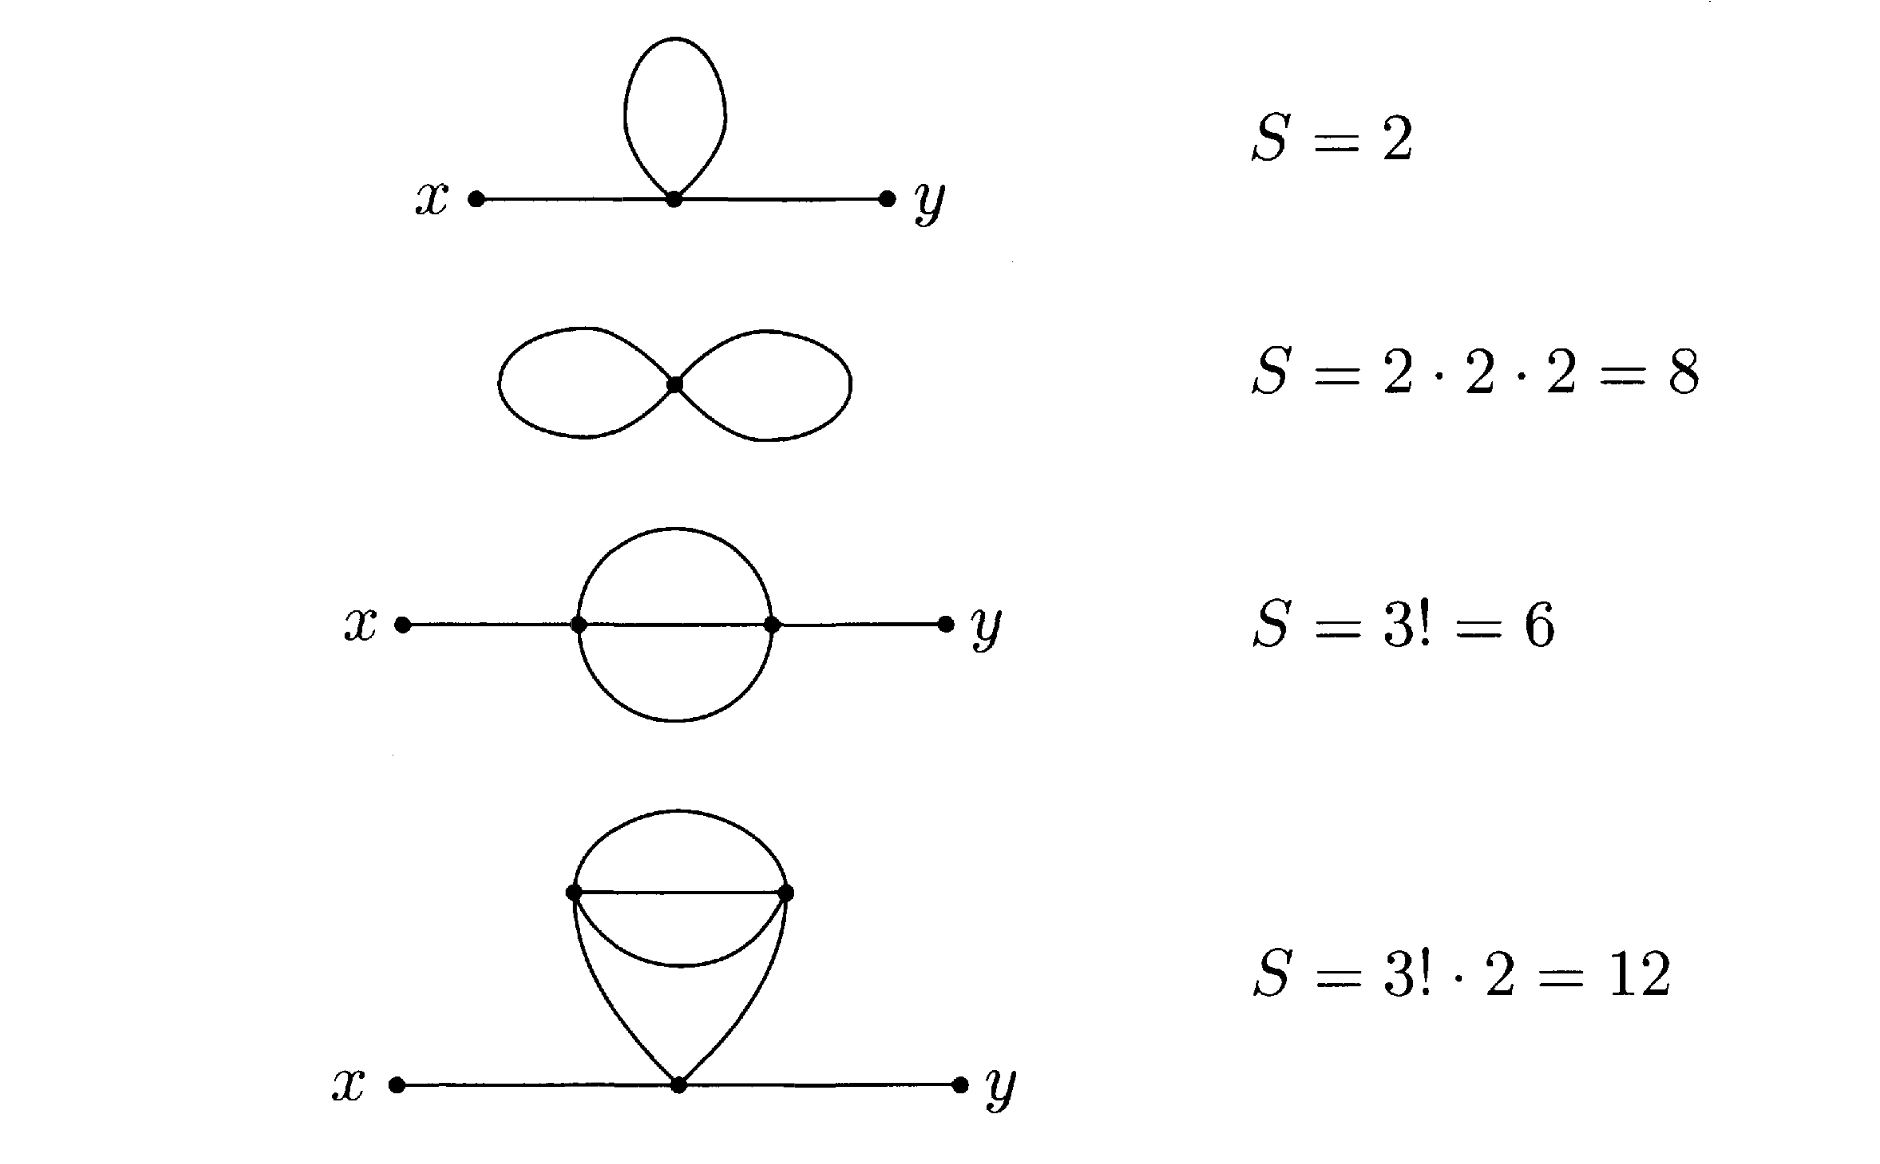
\includegraphics[width=0.9\textwidth]{figures/ex1.png}\tag{4.45} \label{ex1}
\end{equation*}

疑わしいときは、等価な収縮の数を数えることで対称性因子を決めればよい。  

さて、式 (4.31) に戻り、相関関数の分子部分を計算するための規則をまとめよう:

\begin{equation*}
\langle 0|T\{\phi(x)\phi(y)\}\exp\!\left[-i\int dt\, H_I(t)\right]|0\rangle
= \left(\sum_{\text{全ての図}}\right),
\end{equation*}

ここで各図は伝播子、頂点、外部点で構成される。  
このように解析式と図の要素を対応させる規則を \textbf{ファインマンルール} と呼ぶ。  
$\phi^4$ 理論におけるルールは次の通り:

\begin{equation*}
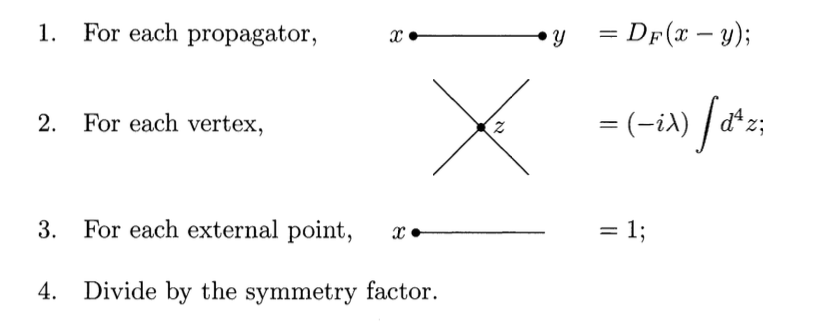
\includegraphics[width=0.9\textwidth]{figures/Frule_ex.png}\tag{4.46} \label{frule_ex}
\end{equation*}


これらの規則の一つの解釈は、頂点因子 $(-i\lambda)$ を「粒子の放出や吸収の振幅」とみなすことである。  
積分 $\int d^4z$ は、その過程が起こりうる全ての点 $z$ について和をとることを指示する。  
これは量子力学の重ね合わせの原理に他ならない。  

従って、各過程が複数の方法で起こり得るならば、その全ての振幅を足し合わせる必要がある。  
最終的な振幅は、伝播子と頂点因子の積をすべての要素について掛け合わせることで得られる.

これらの規則は時空点 $x,y$ で書かれているので、しばしば \textbf{位置空間ファインマンルール} と呼ばれる。  
実際の計算では運動量表示に変換した方が便利である。そこで各伝播子のフーリエ展開を導入する:

\begin{equation*}
D_F(x-y) = \int \frac{d^4p}{(2\pi)^4} \frac{i}{p^2-m^2+i\epsilon} e^{-ip\cdot(x-y)}.
\tag{4.46}
\end{equation*}

これを図式的に表すには、各伝播子に4運動量 $p$ を割り当て、矢印で方向を示す($D_F(x-y)=D_F(y-x)$ なので方向は任意である)。  
4本の線が頂点で交わるとき、$z$ 依存因子の積分は

\begin{equation*}
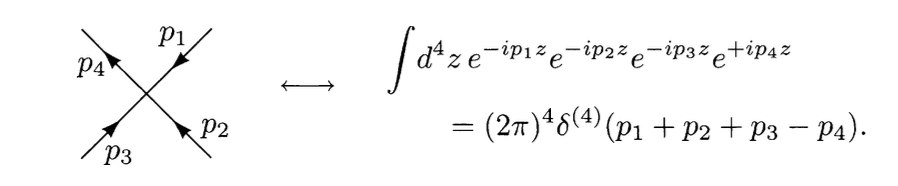
\includegraphics[width=0.9\textwidth]{figures/4.47.png}\tag{4.47} \label{4.47}
\end{equation*}


すなわち、各頂点では運動量が保存される。このデルタ関数が運動量保存則を表す。


\subsection*{運動量空間におけるファインマンルール}

頂点からの積分を用いて、伝播子の運動量積分の一部を実行できる。  
その結果として得られるのが次の \textbf{運動量空間ファインマンルール} である:

\begin{equation*}
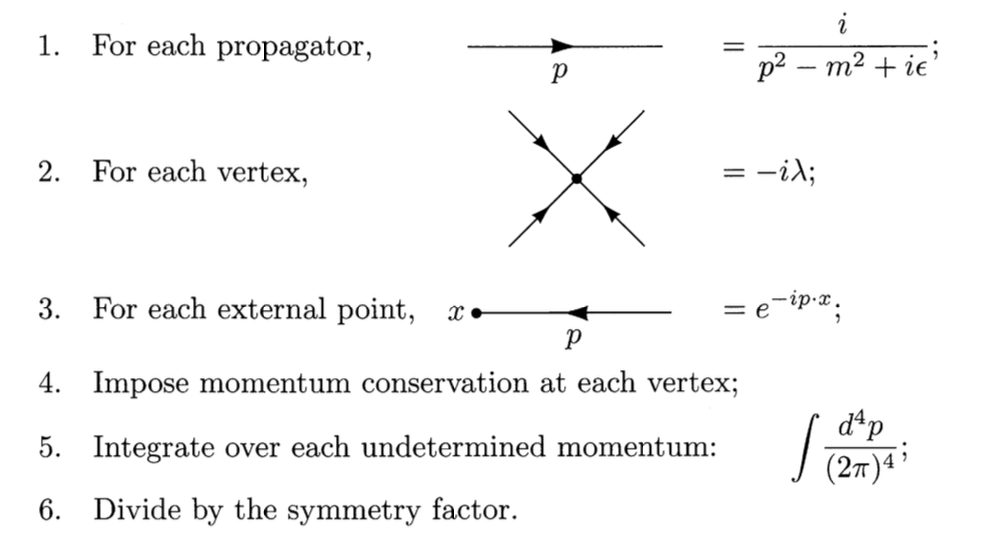
\includegraphics[width=0.9\textwidth]{figures/FR.png}
\end{equation*}

再び、各因子をその部分過程の振幅と解釈できる。積分は重ね合わせの原理から来る。  
外部点の指数因子は、その点に運動量 $p$ をもつ粒子が見いだされる振幅を表す。矢印の向きによっては粒子が出ていく場合か入ってくる場合かが決まる。  

これで相関関数の計算に関する議論はほぼ完了するが、まだいくつかの問題が残っている。  
まず、大きな時間 $T \to \infty(1-i\epsilon)$ はどうなったのか。  
式 (4.43) から始めたこの議論では触れずに済ませたが、式 (4.47) に戻すと、単に $d^4z$ の積分を行う代わりに次のようにすべきである:

\begin{equation*}
\lim_{T \to \infty (1-i\epsilon)} \int_{-T}^T dz^0 \int d^3z \,
e^{-i(p_1+p_2+p_3-p_4)\cdot z}.
\end{equation*}

この指数因子は $z^0 \to \infty$ または $z^0 \to -\infty$ のときに発散してしまう。  
これを防ぐために、$p^0$ に小さな虚部 $i\epsilon$ を与える。これがファインマン境界条件である。  
つまり実軸からわずかに傾いた経路で積分することで $p^0 \propto (1+i\epsilon)$ を実現する。


\begin{equation*}
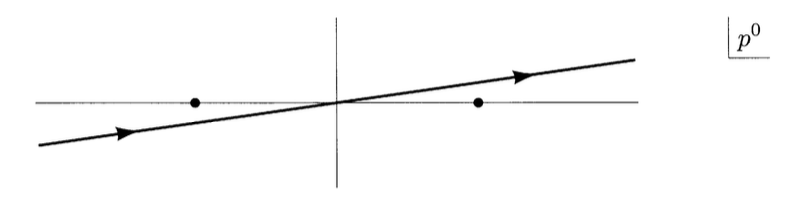
\includegraphics[width=0.9\textwidth]{figures/p0.png}
\end{equation*}

前の式においてT→0の極限を取ると、Tへの明示的な依存性は消えるように見える。しかし、次の図を考えてみる:

\begin{equation*}
    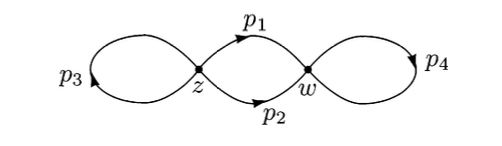
\includegraphics[width=0.8\textwidth]{figures/4.48.png}\tag{4.48} \label{4.48}
\end{equation*}


左の頂点からのデルタ関数は $(2\pi)^4 \delta^{(4)}(p_1+p_2)$ を与える。右の頂点でも自動的に保存則が成立し、$(2\pi)^4\delta^{(4)}(0)$ が出る。  
この奇妙な因子は位置空間に戻ると理解しやすい。単に定数の $d^4w$ にわたる積分:

\begin{equation*}
\int d^4w (\text{const}) \propto (2T)\cdot (\text{Volume of space}).
\end{equation*}


これは「過程 (4.48) が時空内の任意の位置で、$-T$ から $T$ の間いつでも起こり得る」ことを意味している。  
外部点に結びつかない部分、すなわち \textbf{切れた部分} はそれぞれ、このような $(2\pi)^4\delta^{(4)}(0) = 2T\cdot V$ の因子をもつ。  

切れた図からの寄与は、美しい恒等式を使って理解できる。  
すなわち \textbf{切れた図の指数化} である。典型的な図は次のような形をしている:

\begin{equation*}
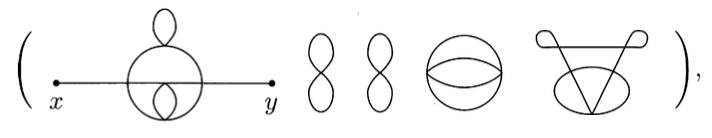
\includegraphics[width=0.9\textwidth]{figures/4.50.png}\tag{4.50} \label{4.50}
\end{equation*}

ここでは $x,y$ に接続した部分と、いくつかの切れた部分が存在する。  
各頂点は偶数本の線をもち、したがって $x,y$ は互いに接続されていなければならない。  

切れた部分を $V_i$ とラベルすると、

\begin{equation*}
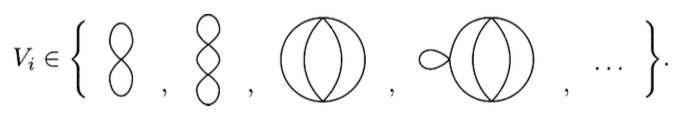
\includegraphics[width=0.9\textwidth]{figures/4.51.png}\tag{4.51} \label{4.51}
\end{equation*}

各 $V_i$ は外部点から切り離されているが、内部では連結している。  
もし図が $n_i$ 個の $V_i$ を含むなら、その値は

\begin{equation*}
(\text{connected 部分の値}) \times \prod_i \frac{1}{n_i!} (V_i)^{n_i}
\end{equation*}

となる。$1/n_i!$ は $n_i$ 個の同一の $V_i$ を入れ替える対称性因子である。  

二点相関関数の式における分子を表す全図形の和は,

\[
\sum_{\text{全ての連結した部分}} 
\sum_{\{n_i\}} \Big( \text{連結部分の値} \Big)
\left( \prod_i \frac{1}{n_i!} (V_i)^{n_i} \right),
\]

ここで $\{n_i\}$ は非負整数の順序付き集合を表す。  
和を整理すると、

\[
= \left( \sum_{\text{connected}} \right)
\times \sum_{\{n_i\}}
\left( \prod_i \frac{1}{n_i!}(V_i)^{n_i} \right).
\]

さらに展開すると、

\[
= \left( \sum_{\text{connected}} \right)
\times \left( \sum_{n_1} \frac{1}{n_1!} V_1^{n_1} \right)
\left( \sum_{n_2} \frac{1}{n_2!} V_2^{n_2} \right)
\left( \sum_{n_3} \frac{1}{n_3!} V_3^{n_3} \right) \cdots
\]

\[
= \left( \sum_{\text{connected}} \right)
\times \prod_i \left( \sum_{n_i} \frac{1}{n_i!} V_i^{n_i} \right)
\]

\[
= \left( \sum_{\text{connected}} \right)
\times \prod_i \exp(V_i)
\]

\[
= \left( \sum_{\text{connected}} \right)
\times \exp\!\left(\sum_i V_i\right).
\tag{4.52}
\]

したがって、全ての図の和は「連結した図の和」$\times$「切れた図の和の指数」である。  
図式的には次の恒等式になる:

\begin{equation*}
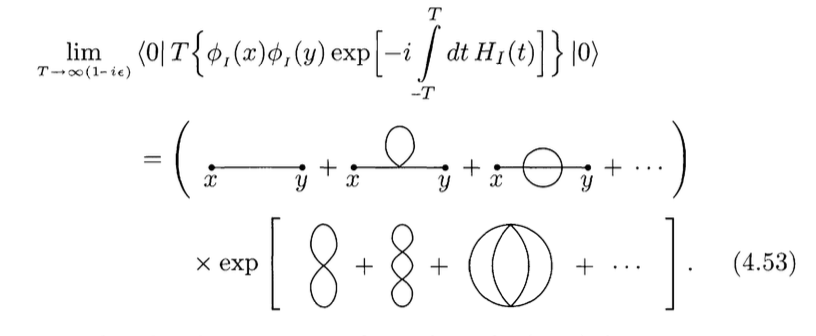
\includegraphics[width=0.9\textwidth]{figures/4.53.png}\tag{4.53} \label{4.53}
\end{equation*}

分母についても同様に考えると、指数が打ち消され、最終的に次を得る:

\begin{equation*}
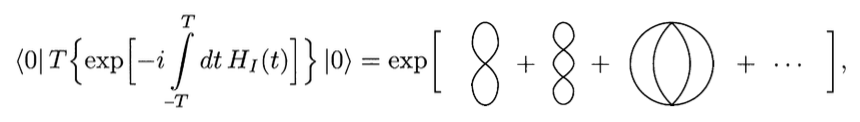
\includegraphics[width=0.9\textwidth]{figures/4.53a.png}
\end{equation*}


例えば、

\begin{equation*}
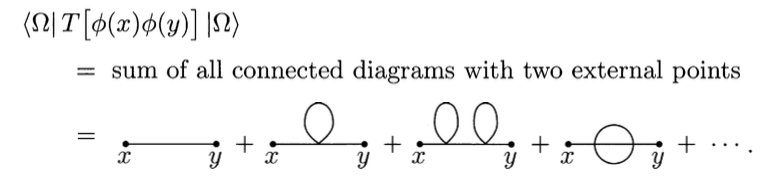
\includegraphics[width=0.9\textwidth]{figures/4.54.png}\tag{4.54} \label{4.54}
\end{equation*}

ここで少し立ち止まり、物理的解釈を考える。  
式 (4.30) に戻ると、

\[
\lim_{T\to\infty(1-i\epsilon)}
\langle 0|T\{\phi(x)\phi(y)\}\exp[-i\int_{-T}^T dt\, H_I(t)]|0\rangle
= \langle \Omega|T\{\phi(x)\phi(y)\}|\Omega\rangle
\cdot \lim_{T\to\infty(1-i\epsilon)} |\langle 0|\Omega\rangle|^2 e^{-iE_0(2T)}.
\]

$T$ に依存する部分だけを見ると、

\[
\exp\!\left(\sum_i V_i\right)
\propto \exp[-iE_0(2T)].
\tag{4.55}
\]

各切れた図 $V_i$ は因子 $(2\pi)^4\delta^{(4)}(0)=2T\cdot V$ を含むため、これにより基底状態のエネルギー密度 $E_0/V$ の公式が得られる:

\begin{equation*}
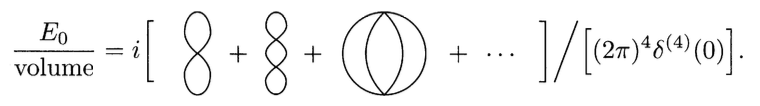
\includegraphics[width=0.9\textwidth]{figures/4.56.png}\tag{4.56} \label{4.56}
\end{equation*}

右辺が $T$ や体積に依存しないことは重要である。特に $E_0$ が体積に比例することを保証する。  

これで二点相関関数の議論は完了する。  
より高次の相関関数への拡張は単純である:

\[
\langle \Omega|T\{\phi(x_1)\cdots \phi(x_n)\}|\Omega\rangle
= \Big(\text{$n$ 個の外部点をもつ連結図の和}\Big).
\tag{4.57}
\]

ここで「切れた図」とは「外部点に結びつかない部分」を意味する。  
これは式 (4.51) で扱ったものと同じである。しばしば「真空バブル (vacuum bubbles)」と呼ばれる。

高次の相関関数では、図は別の意味で「切断される」こともある。  
例えば四点関数を考えよう:

\begin{equation*}
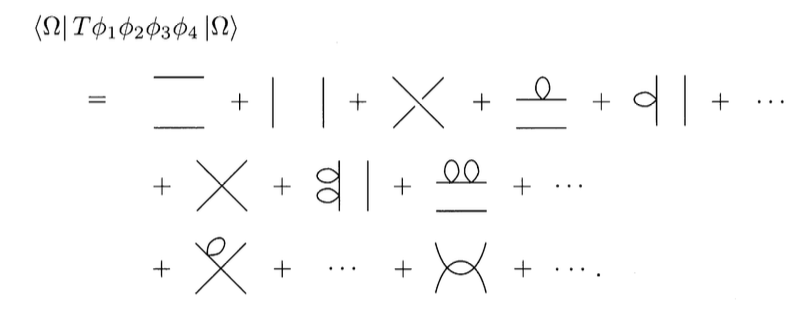
\includegraphics[width=0.9\textwidth]{figures/4.58.png}\tag{4.58} \label{4.58}
\end{equation*}

このような多くの図において、外部点同士が互いに切り離されている。  
そのような図は指数化したり因数分解したりしないが、振幅には寄与する。  
これは完全に連結した図(任意の点が線をたどることで他の任意の点に到達できるもの)と同様である。  


さらに注意すべきは、$\phi^4$ 理論においては奇数個の場の相関関数はすべて消えることである。  
なぜなら、外部点の数が奇数の許容された図を描くことはできないからである。  
ウィックの定理に立ち返ればこれも理解できる。  
相互作用ハミルトニアン $H_I$ は偶数個の場を含んでいるため、摂動展開の各項に現れる相関関数も常に奇数個の場を含むことになる。  
しかし奇数個の場を完全に縮約することは不可能であり、非零の真空期待値をもつのは完全に縮約された項だけだからである。








\end{document}
